\section{Datenquellen und Reproduzierbarkeit}
\label{app:evidence_availability}

\subsection{Quellen und Verfügbarkeit}
\label{app:evidence_sources}

Die zentrale Sammlung \emph{Edge AI Performance and Energy Results}~\cite{edgeAIResults2026} enthält die in dieser Dissertation verwendeten numerischen Eingaben und die Analysesoftware. Tabelle~\ref{tab:appendix:central_sources} gibt die wichtigsten Einstiegspunkte an. Der Einsatzvergleich, der gepaarte Vergleich der Ausführungsmodule und die umfassendere Graphenauswertung stützen sich auf die in Kapitel~\ref{sec:evaluation} beschriebene Kampagne. Unabhängige Energie- und Laufzeitversuche verfügen über eigene Messprotokolle.

\begin{table}[!htb]
\centering\small\TableSetup
\caption{Quellenübersicht. Pfade beziehen sich auf das zentrale Ergebnisrepositorium.}
\label{tab:appendix:central_sources}
\begin{tabularx}{\linewidth}{@{}L{2.7cm}Y@{}}
\toprule
Beweismittel & Einstiegspunkt des Repositorys \\
\midrule
Energiemessung & \path{results/energy-measurement/}: Rekonstruktion, Spektren, Messgerätevergleiche, Kalibrierung und Protokollkontrollen. \\
Vergleich der Ausführungskonfigurationen & \path{results/split-inference/}: Qualität, Zeitablauf, Energie, Wiederholungen und Full-Referenzen. \\
Auswahl und unterstützende Studien & \path{results/supplementary-studies/}: Rangfolgen der Kandidaten, angepasste Werte, stufenweise Auswahl und Laufzeitprüfungen. \\
Zuordnung der Veröffentlichungen & \path{publications/}: Quellkarten für Manuskripte und Dissertationen. \\
Reproduktions\-software & \path{scripts/} und \path{software/}: Analysebefehle und gespeicherte Softwarequellen. \\
\bottomrule
\end{tabularx}
\end{table}

Der fertige Datensatz wurde in der Revision \path{0a45553836acf91a4faad80adc1779af99591b53} veröffentlicht. Die numerischen Analysen basieren auf \path{aed301819663b5fa27bd5731fb74fef3e46ee927}. Die exportierten Abbildungen der Dissertation sowie die Software werden in der Revision \path{3cc8ad92fb1a58e6e793561e489d323e19f15a01} veröffentlicht. Ihre Quell- und Ausgabe-Hashes sind im LaTeX-Projekt erfasst. Die separate Studie mit kontinuierlicher Eingabe verwendet die Revision \path{6ebc90deca31c9890d7ebccd7fd2981f8bda0c96}~\cite{v49Confirmation2026}.

Große Modelle, Hersteller-Binärdateien, Datensatzbilder, vollständige Vorhersagen und Rohwellenformen werden in externen Erfassungsarchiven aufbewahrt. Die Wiederholung physikalischer Messungen erfordert diese Eingaben, ihre Softwareumgebungen sowie die Zielsysteme. Ihre Verfügbarkeit und ihre Weiterverbreitungsrechte unterscheiden sich von denen der veröffentlichten numerischen Exporte. Die nachstehenden Reproduktionsbefehle erzeugen Analysen aus aufgezeichneten Ergebnissen neu, ohne die Hardware-Messungen zu wiederholen.

\subsubsection{Energie- und Manuskriptquellen}
\label{app:energy_evidence_v43}

Die drei Manuskripte des Autors enthalten die Energiestudien und die Split-Selection-Studie~\cite{mika2026parmaEnergy,mika2026timEnergy,mika2026mlsysSplit}. Die Selektionsanalyse folgt dem abschließenden MLSys-Manuskript. Kapitel~\ref{sec:energy} verwendet die gesamte FP16-Population mit allen fünfzehn Elementen sowie die korrigierte native Referenzrekonstruktion. Die numerischen Eingabedaten sind unter \path{results/energy-measurement/} archiviert, die zugehörigen Quellen der Dissertation unter \path{results/supplementary-studies/dissertation-v56/}. Die Referenz~\cite{energyEvidence2026} verweist auf die früher festgelegte Sammlung von Energiedaten. Das aktuelle Repository enthält deren Eingabedaten sowie die Exporte aus der Dissertation.

Numerische Exporte geben die berichteten Zusammenfassungen wieder. Spektralschätzung und Wellenformrekonstruktion erfordern zusätzlich die Rohaufzeichnungen oder verifizierten Caches sowie deren Erfassungseinstellungen. Rekonstruktion, physikalische Abtastung und Vergleiche mit eingesetzten Messgeräten testen unterschiedliche Effekte. Kapitel~\ref{sec:energy} definiert deren elektrische und zeitliche Geltungsbereiche.

\subsection{Reproduktion von Abbildungen und Tabellen}
\label{app:current_selection_reproduction}

Nach dem Auschecken der oben genannten Überarbeitung des Abbildungsexports generiert der folgende Befehl die englischen Publikationsartefakte aus den aufgezeichneten Messungen neu:
\begin{lstlisting}[language={},basicstyle=\ttfamily\footnotesize]
python3 scripts/reproduce_current.py \
  --output local-output/current --languages en
\end{lstlisting}
Die Installation der Abhängigkeiten wird in \path{scripts/README.md} beschrieben. Zu den in \path{scripts/split-inference/requirements-r30.txt} festgelegten Abhängigkeiten gehören pandas und SciPy für die Datenverarbeitung und numerische Auswertung \cite{mckinney2010pandas,virtanen2020scipy} sowie Matplotlib für Diagramme und PyMuPDF für die PDF-Verarbeitung \cite{hunter2007matplotlib,pymupdf_docs}. Die Datei \path{results/ACTIVE_GENERIC420.json} identifiziert die Kampagneneingaben. Die gepaarten, umfassenderen Generic- und stufenweisen Analysen sind unter \path{results/supplementary-studies/rq2-native-scope-20261027/}, \path{rq3-generic420-detector-corrected-20261027/} und \path{staged-selection/} enthalten.

Der Abbildungsgenerator für Dissertationen verwendet dieselben numerischen Eingaben:
\begin{lstlisting}[language={},basicstyle=\ttfamily\footnotesize]
python3 scripts/dissertation/export_thesis_selection.py \
  --output local-output/thesis-en \
  --figure-profile dissertation
\end{lstlisting}
Der Auswahl-Exporter generiert die aktuellen Ergebnisabbildungen und -tabellen neu. Dreizehn frühere englische Abbildungen bleiben als feste Publikationsexporte mit ihren ursprünglichen Quellzuordnungen und Hashes erhalten. Sie werden mit folgendem Befehl kopiert und überprüft:
\begin{lstlisting}[language={},basicstyle=\ttfamily\footnotesize]
python3 scripts/dissertation/export_frozen_thesis_figures.py \
  --output local-output/thesis-en-fixed
\end{lstlisting}
Diese festgelegten Exporte bewahren die früheren Layouts. Durch das Kopieren werden die zugrunde liegenden Analysen nicht erneut ausgeführt. Konzeptionelle Diagramme stammen aus den mitgelieferten englischen draw.io-Quellen \cite{drawio_documentation} und verwenden den Exporter unter \path{scripts/dissertation/drawio/}. Das LaTeX-Projekt enthält die endgültigen PDF-Abbildungen, Tabellen und Texte, die zum Erstellen des Dokuments benötigt werden. Die Neuberechnung von Qualitätsmetriken oder Energieintegralen erfordert die separaten Vorhersage- oder Wellenformdatensätze.

\subsubsection{Überprüfung der gespeicherten numerischen Eingaben}
\label{sec:review:offline_audit}

Bei einer früheren Offline-Prüfung wurden 227 numerische Dateien und 38 Bestätigungsausgaben Byte für Byte aus ihren eingefrorenen Eingaben reproduziert~\cite{v53OfflineAudit2026}. Zudem wurden Modelloperatoren, Bewertungsgrößen und ausgewählte Vorhersageidentitäten überprüft. Gespeicherte Bootstrap-Werte wurden wiederverwendet; Inferenz, Qualitäts-Resampling und physikalische Erfassung wurden nicht wiederholt. Die aktuellen Auswahlexporte verfügen über eigene Eingabemanifeste und numerische Prüfungen. Diese Prüfungen ermitteln, welche aufgezeichneten Eingaben zu einem Ergebnis geführt haben. Die Reproduzierbarkeit auf Hardwareebene hängt zudem von den kompilierten Artefakten, den Laufzeitversionen und den Geräteeinstellungen ab.

\subsection{Messprotokolle und Messumfang}
\label{app:current_evidence_limits}

Jede Konfiguration verknüpft die kompilierten Artefakte, die Laufzeitumgebung, die Qualitätsbewertung und die Durchsatzbeobachtungen. Durchsatzaufzeichnungen enthalten die Aufwärmphase, die Anzahl der abgeschlossenen Aufgaben und das gemessene Intervall. Energieaufzeichnungen identifizieren zusätzlich den elektrischen Kanal, die Kalibrierung und das Integrationsintervall. Anhang~\ref{app:split_reproduction} enthält die Einstellungen für die Ausführungskonfigurationen und Auswahl.

Der primäre Vergleich wendet die numerische 5\%-Regel für den relativen Qualitätsverlust gegenüber der CPU-Referenz an und stützt sich dabei auf ungerundete Werte. Die beobachteten Wiederholungsbereiche beschreiben Abweichungen zwischen den Durchläufen. Sie berücksichtigen weder die Unsicherheit bei der Gewinnerauswahl noch alle systematischen Messeffekte. Da einige historische Aufzeichnungen zu Compilern, Auswertungsprogrammen und Gerätestatus unvollständig sind, kann das Archiv nicht jede frühere Ausführungsumgebung rekonstruieren.

Kalibrierung, separate Verifikation und Validierung unter realer Last werden in Kapitel~\ref{sec:energy} beschrieben. Die Bestätigung der beibehaltenen Hardware identifiziert den Kanal CH0 und den eingebauten ADS7953. Die Bezeichnung ADS7952 in einer Quelle ist ein Dokumentationsfehler. Aufbauspezifische Kalibrierungsprofile bewahren die auf die Energiebeobachtungen angewendeten Koeffizienten.

Abbildung~\ref{fig:energy:current_verification} ergänzt die in Abschnitt~\ref{sec:energy:verification} zusammengefasste Prüfung der Stromkalibrierung. Sie zeigt die einzelnen Abweichungen von der Fluke-Referenz im unabhängigen Verifikationsdurchlauf.

\begin{figure}[!htb]
 \centering
 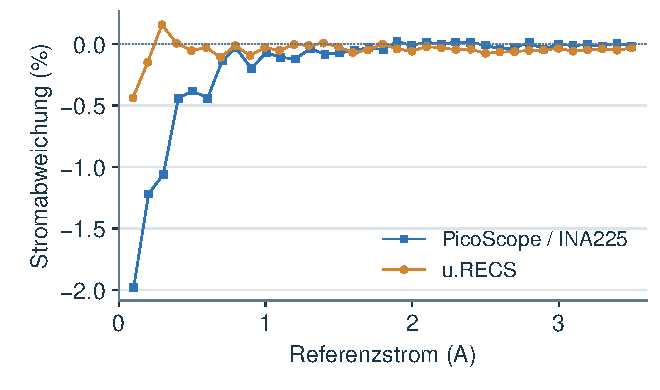
\includegraphics[width=247.68bp]{9_resources/04_energiemessung/current_verification.pdf}
 \caption[Unabhängige Residuen der Stromverifikation.]{Vorzeichenbehaftete Stromabweichungen von der Fluke-Referenz im separaten Durchlauf der Verifikation: 35 von Null verschiedene Werte pro Pfad, einschließlich der größeren Restabweichungen bei niedrigen Stromstärken. Neu gezeichnet aus den archivierten Verifikationszeilen \cite{energyEvidence2026}.}
 \label{fig:energy:current_verification}
\end{figure}

\subsection{Ergänzende Angaben zu den Energieexperimenten}
\label{app:energy_study_details}

Die folgenden Angaben ergänzen die experimentellen Untersuchungen in Abschnitt~\ref{sec:energy:measurement_studies} und die Verifikation in Abschnitt~\ref{sec:energy:verification}. Sie gelten jeweils für die zugehörige Versuchsreihe.

\emph{Spannungsmodell der Referenzmessungen.} Das Spannungsmodell aus Gleichung~\ref{eq:energy:voltage_model} wurde für Ströme zwischen 0 und \SI{3.5}{\ampere} charakterisiert. Die aus den dokumentierten Kalibrierungsmessungen übernommenen Koeffizienten betragen $a_U\approx\SI{19.062607}{\volt}$ und $b_U\approx-\num{0.07444582}$~V/A \cite{energyEvidence2026,v49Confirmation2026}. Für Ströme außerhalb des untersuchten Bereichs wird das Modell linear extrapoliert. Die Vergleiche mit zwei Oszilloskopen verwenden dieses Spannungsmodell für beide Pfade und bewerten daher die Übereinstimmung der Strompfade. Andere Versuchsreihen verwenden ihre aufgezeichneten Spannungsmesswerte oder Schätzwerte. Der für die Spannungsmessung verwendete PicoScope-Eingang hat eine Bandbreite von \SI{20}{\mega\hertz} \cite{pico4224A}.

\emph{Leistungsskalierung beim Messgeräte- und Dauervergleich.} Die Untersuchung mit dem Jetson und der \textit{u.RECS}-Messung verwendet den aufbauspezifischen Faktor
\begin{equation}
 P_{\mathrm{Jetson,corr}}=c_{\mathrm{setup}}U_{\mathrm{est}}I_{\mathrm{cal}},
 \qquad c_{\mathrm{setup}}\approx\num{0.97}.
 \label{eq:energy:jetson_setup_factor}
\end{equation}
Der Faktor $c_{\mathrm{setup}}$ wurde aus den mittleren Abweichungen zur Referenz in den beiden Pilot-Benchmarks variables YOLO und GEMM-FP16 abgeleitet. Für die nachfolgenden Benchmark-Vergleiche blieb er unverändert \cite[pp.~65--66]{wachsmuth2026masterarbeit}. Die Shelly-Messwerte werden mit ihrer empirisch ermittelten Skalierung ausgewertet. Diese Skalierung gleicht die unterschiedlichen elektrischen Messgrenzen der Messsteckdose und der Messung an der Modul- oder Beschleunigerversorgung nicht an.

Die Dauerstudie umfasst sieben Arbeitslasten bei zehn Dauerwerten von 5 bis 600~s mit jeweils 15 Wiederholungen pro Dauer. Sowohl die u.RECS-Messung als auch das PicoScope zeichnen mit 2~kS/s auf. Nach der Korrektur weichen die angegebenen Werte der mittleren Leistungsaufnahme für \textit{u.RECS} um höchstens etwa \num{0.5}\% vom PicoScope-Referenzwert ab. Dies validiert die korrigierte Methode bei realen Arbeitslasten über die getesteten Laufzeiten hinweg \cite[pp.~64--67]{wachsmuth2026masterarbeit}.

\emph{Modelle, Rechenlasten und Datensatzbezeichnungen.} Die FP16-Messungen mit langen Zeitfenstern bilden eine eigenständige Versuchsreihe. Die Jetson-Versuche zur Wiederholbarkeit bei unterschiedlichen Erfassungsraten verwenden GEMM und YOLO mit TensorRT in FP32, FP16 und INT8, YOLO mit variabler Aktivität sowie Gemma3-12B über Ollama \cite{ollama_runtime,mika2026parmaEnergy}. Gemma3-4B und Gemma3-12B werden aufgrund ihrer unterschiedlichen Modellgrößen getrennt ausgewertet. Für die Hailo-10-Messungen werden die in den Messdaten hinterlegten Bezeichnungen GEMM, YOLO, variable-YOLO und LLM verwendet. Einige ältere Aufzeichnungen enthalten nur unvollständige Angaben zu Eingabedaten, Modellversionen und Kompilierungseinstellungen. Die Auswertung bezieht sich daher jeweils auf die dokumentierte Versuchsreihe. Geräteübergreifende Vergleiche mit festgelegten Modellen, Laufzeiteinstellungen und einer definierten Anzahl vollständig verarbeiteter Aufgaben werden in den Inferenzkapiteln behandelt \cite{energyEvidence2026,edgeAIResults2026}.

\emph{Wiederholbarkeit bei unterschiedlichen Erfassungsraten.} Diese Untersuchung umfasst acht Jetson- und vier Hailo-Reihen mit insgesamt 323 Ratengruppen und \num{4842} auswertbaren Ergebnissen. Eine Ratengruppe enthält die wiederholten Ausführungen derselben Berechnung bei einer festgelegten Erfassungsrate. Tabelle~\ref{tab:energy:direct_rates} unterscheidet die Streuung innerhalb dieser Gruppen von den Unterschieden zwischen den Gruppen.

Der Variationskoeffizient (\emph{coefficient of variation}, CV) setzt die Populationsstandardabweichung der gemessenen Energien ins Verhältnis zu ihrem Mittelwert und wird in Prozent angegeben. Für den Vergleich zwischen den Raten wird zunächst der gleichgewichtete Mittelwert aller Ratengruppenmittelwerte gebildet. Die Verschiebung bezeichnet die relative Abweichung eines Gruppenmittelwerts von diesem Vergleichswert. Angegeben werden jeweils der größte CV und die betragsmäßig größte Verschiebung innerhalb einer Versuchsreihe.

\begin{table}[!htb]
\centering\small\TableSetup
\caption[Streuung innerhalb einer Erfassungsrate und Unterschiede zwischen den Raten.]{Größter Variationskoeffizient der Energie innerhalb einer Erfassungsrate und größte absolute relative Abweichung eines Ratengruppenmittelwerts vom gleichgewichteten Mittel aller Ratengruppen. Die Anzahl der Durchläufe umfasst nur Aufzeichnungen mit einem auswertbaren Lastintervall \cite{edgeAIResults2026}.}
\label{tab:energy:direct_rates}
\begin{tabular}{@{}llrrS[table-format=2.2]S[table-format=2.2]@{}}
\toprule
Plattform & Arbeitslast & Raten & Durchläufe & {\shortstack{Max. CV\\(\%)}} & {\shortstack{Max. Verschiebung\\(\%)}} \\
\midrule
Jetson & GEMM-FP32 & 27 & 405 & 0.37 & 0.40 \\
Jetson & GEMM-FP16 & 27 & 405 & 0.73 & 2.08 \\
Jetson & GEMM-INT8 & 27 & 405 & 0.63 & 1.69 \\
Jetson & YOLO-FP32 & 26 & 390 & 0.41 & 0.89 \\
Jetson & YOLO-FP16 & 27 & 405 & 0.44 & 0.25 \\
Jetson & YOLO-INT8 & 27 & 405 & 0.73 & 0.31 \\
Jetson & Variables YOLO & 27 & 405 & 0.49 & 0.56 \\
Jetson & Gemma3-12B & 27 & 405 & 0.58 & 1.66 \\
Hailo & GEMM & 27 & 405 & 0.68 & 1.48 \\
Hailo & YOLO & 27 & 405 & 1.01 & 1.20 \\
Hailo & Variables YOLO & 27 & 405 & 9.45 & 6.74 \\
Hailo & LLM & 27 & 402 & 46.06 & 24.30 \\
\bottomrule
\end{tabular}

\end{table}

\emph{Kontrollversuch zum Einfluss der Erfassungsrate.} Der Kontrollversuch verwendet zwölf FP16-Ausführungen mit derselben TensorRT-Engine, jeweils 250 abgeschlossenen Inferenzen, unveränderter \emph{Spin-Wait}-Einstellung und einer Pause von 120 Sekunden zwischen Prozessende und nächstem Start. Für $A=2$~kS/s und $B=5$~MS/s werden in zwei Messsitzungen die Reihenfolgen ABBAAB und BAABBA verwendet. Damit kommt jede Rate über beide Sitzungen hinweg an jeder Position einmal vor.

Ein additives lineares Modell berücksichtigt die Erfassungsrate, die Messsitzung und die Position innerhalb der Reihenfolge. Die Position wird als kategoriale Variable behandelt. Die Modellmatrix besitzt acht linear unabhängige Spalten. Bei zwölf Beobachtungen verbleiben damit vier Restfreiheitsgrade für die Schätzung der nicht durch das Modell erklärten Streuung. Das Modell setzt additive Sitzungsunterschiede und gemeinsame Positionseffekte voraus. Wechselwirkungen zwischen diesen Einflussgrößen werden nicht geschätzt.

Die zweiseitigen 95\%-Konfidenzintervalle werden mit der $t$-Verteilung und vier Restfreiheitsgraden berechnet. Die geschätzten Änderungen von 5~MS/s gegenüber 2~kS/s sowie die Intervallgrenzen werden durch den beobachteten Mittelwert bei 2~kS/s geteilt und in Prozent angegeben. Die Intervalle gelten unter den Modellannahmen für diese zwölf Durchläufe. Sie stellen weder einen formalen Äquivalenztest noch einen Nachweis der absoluten Messgenauigkeit dar \cite{mika2026timEnergy,energyEvidence2026}.

Die als „Hailo LLM“ aufgezeichnete Reihe erreicht einen maximalen Energie-CV von etwa 46\,\% und eine größte Gruppenabweichung von etwa 24\,\%. Drei von 405 Aufzeichnungen liefern kein auswertbares Lastintervall. Variables Hailo-YOLO erreicht einen maximalen CV von \num{9.45}\,\%, während die kontinuierlichen GEMM- und YOLO-Ausführungen deutlich weniger streuen. Aufgrund der oben beschriebenen Lücken in den Modell- und Kompilierungsaufzeichnungen lässt sich das beobachtete Verhalten der Hailo-LLM-Reihe nicht eindeutig einer konkreten Modellarchitektur zuordnen \cite{energyEvidence2026,edgeAIResults2026}.

\emph{Prüfung der automatischen Intervallerkennung.} Die angeforderte Dauer und die resultierende Energie beeinflussen den Schwellenwert nicht. Die relativen Schwellen \num{0.4} und \num{0.6} prüfen die Empfindlichkeit gegenüber der primären \num{0.5}-Regel. Wird kein Intervall erkannt, bleibt das Ergebnis fehlend. Die archivierte Methodenbeschreibung enthält alle Erkennungsbedingungen und den Umgang mit Endzeitstempeln \cite{energyEvidence2026}.

Für die Untersuchung wechselnder Aktivität auf Hailo wird das explizit aufgezeichnete Intervall einschließlich des zusätzlichen Randbereichs verwendet. Die Aufzeichnungen tragen die Bezeichnung \texttt{variable-YOLO}. Das anhaltende Anfangsniveau erlaubt hier keine zuverlässige Erkennung des Lastbeginns. Diese Intervallwahl gilt für alle zugehörigen Raten- und Dauerreihen. Ihr Einfluss auf den Vergleich von mittlerer Leistungsaufnahme und Energie wird in Abschnitt~\ref{sec:energy:verification} anhand der unterschiedlich langen Messintervalle erläutert \cite{mika2026timEnergy,energyEvidence2026}.

\emph{Sensitivitätsprüfung der Rekonstruktion.} Eine zusätzliche Prüfung reduziert die Daten vor der Rekonstruktion auf 1~MS/s. Dabei bleibt das Integral der vollständigen Aufzeichnung erhalten, einige anschließend berechnete Integrale mit niedriger Abtastrate ändern sich jedoch. Die Hauptergebnisse verwenden deshalb die ursprünglichen Daten mit 5~MS/s. Der alternative Weg dient als dokumentierte Sensitivitätsprüfung \cite{energyEvidence2026}.

\emph{Segmentierung bei der Spektralschätzung.} Für den Vergleich von Energieintegration und spektraler Abdeckung bei langen Messintervallen werden aus allen 15 FP16-Aufzeichnungen aufeinander abgestimmte viersekündige Aktiv- und Leerlaufintervalle mit 1~MS/s ausgewertet. Einsekündige Hann-Segmente mit 50\% Überlappung ergeben jeweils sieben Segmente. Diese Vorverarbeitung ist von der Energierekonstruktion der Originalkurve getrennt \cite{mika2026timEnergy,energyEvidence2026}. Bei der Spektralanalyse auf Hailo verwendet die Schätzung Hann-Segmente mit \num{1048576} Abtastwerten, 50\% Überlappung und die dokumentierte Umrechnung in Leistung. Die Frequenzperzentile werden für jede Aufzeichnung einzeln berechnet und anschließend aggregiert \cite{mika2026timEnergy}.

\emph{Offset-Korrektur beim Vergleich der Oszilloskope.} Die Aufzeichnungen zur Objekterkennung in FP32 (Datensatzbezeichnung \texttt{YOLO-FP32}) verwenden eine separate additive Korrektur des Tektronix-Stromoffsets. Die Rohwerte und der Korrekturdatensatz bleiben erhalten. Diese Korrektur nutzt Informationen aus dem anderen Messpfad. Die daraus resultierende Übereinstimmung unterscheidet sich daher von einer unabhängigen Verifikation \cite{energyEvidence2026}.

Die Wahl des Messverfahrens richtet sich danach, ob die Gesamtenergie einer Ausführung oder einzelne schnelle Leistungsschwankungen untersucht werden sollen. Tabelle~\ref{tab:energy:measurement_choice} ordnet diesen Fragestellungen geeignete Messpfade und die erforderlichen Prüfungen zu.

\begin{table}[!htb]
\centering\small\TableSetup
\caption{Messoptionen für die in Kapitel~\ref{sec:energy} untersuchten Fragestellungen. Numerische Ergebnisse behalten ihre getestete Arbeitslast, ihre Messgrenzen und ihr Intervall bei.}
\label{tab:energy:measurement_choice}
\begin{tabularx}{\linewidth}{@{}L{3.0cm}L{3.5cm}Y@{}}
\toprule
Frage & Nützliche Beobachtung & Erforderliche Überprüfung \\
\midrule
Energie im Ausführungsintervall & Kalibrierter DC-Eingang des vollständigen Knotens & Abgeschlossene Arbeiten, ursprüngliche Trace-Kontinuität, übereinstimmender Start- und Endzeitpunkt und Kanal-Verifikation \\
Energie über ein kurzes Ereignis & Externe DC-Referenz mit hoher Rate, gefolgt von einer Ratenrekonstruktion & Fehler bei der vorgesehenen Dauer und den Gitter-Offsets. Das 1\%-Persistenzminimum für Jetson bei 100~ms beträgt 80~kS/s \\
Schnelle Leistungsschwankungen & Externe Erfassung mit hoher Rate & Gemessene spektrale Abdeckung und analoge Antwort. Die FP16-Entscheidungen zur 95/99\%-Abdeckung liegen bei 125/160~kS/s \\
Überwachung zugänglicher Module/Karten & Eingebettete DC-Messung oder validierte Telemetrie & Elektrische Messgrenze an der Versorgungsschiene, tatsächliches Aktualisierungsverhalten und paarweise Übereinstimmung für das beabsichtigte Aktivitätsmuster \\
Aus der Stromversorgung entnommene Energie & AC-seitige Messung der angegebenen Anordnung & Enthaltene Lasten, Umwandlungsverluste, das tatsächliche Intervall und etwaige empirische Skalierungen \\
\bottomrule
\end{tabularx}
\end{table}

\subsection{Kalibrierung des Systemeingangs und aufgezeichneter Messbereich}
\label{app:deployment_energy_path}

Der Einsatzvergleich gibt die Energie am Eingang jedes bestückten Systems an, einschließlich des Leerlaufverbrauchs und nachgelagerter Umwandlungsverluste. Die Kalibrierungsdatensätze identifizieren CH0 und die Verbindung \texttt{9V\_20V\_IN\_after\_R16\_to\_GND}. Für H8, H10 und DeepX gelten separate Profile (Tabelle~\ref{tab:appendix:input_profiles}). Ihre Quelldatensätze werden unter \path{results/energy-measurement/data/calibration/split-setups/}~\cite{edgeAIResults2026,v49Confirmation2026} gespeichert.

\begin{table}[!htb]
\centering\small\TableSetup
\caption{Aufbauspezifische Leistungs-/Energiefaktoren, erfasst am 4. September 2026. Jeder Faktor wird einmal nach den Strom- und Spannungskorrekturen angewendet.}
\label{tab:appendix:input_profiles}
\begin{tabular}{@{}lr@{}}
\toprule
Einrichtung & Faktor $s$ \\
\midrule
Hailo-8 & \num{0.913634} \\
Hailo-10H & \num{0.896397} \\
DeepX DX-M1 & \num{0.903508} \\
\bottomrule
\end{tabular}
\end{table}

Der H10-Datensatz verwendet eine Erfassungsrate von 2 kS/s und 30-Sekunden-Aufnahmen. Seine beiden hinzugefügten Lasten wiesen gemessene Strom-Spannungs-Paare von \num{0.509}~A/\num{18.55}~V und \num{1.01}~A/\num{18.29}~V auf. Benachbarte Leerlaufbeobachtungen eliminieren die Dauerlast bei der Anpassung der inkrementellen Leistungsaufnahme. Dies dient der Überprüfung der lastabhängigen Skalierung. Es handelt sich nicht um eine unabhängige Messung des absoluten Offsets des gesamten Systems. Die Validierung des ursprünglichen Spannungsmodells ist in Abschnitt~\ref{sec:energy:verification} beschrieben.

Bei den Split-System-Messungen kombiniert die beibehaltene Berechnung die Stromkorrektur, das Spannungsmodell und die aufbau-spezifische Leistungsskalierung wie folgt:
\begin{equation}
 \begin{aligned}
 I&=g\left(\frac{r}{1000}+o\right),\\
 U&=a_U+b_UI,\\
 P&=c_{\mathrm{setup}}\,s\,I\,U.
 \end{aligned}
 \label{eq:energy:split_calibration_chain}
\end{equation}
Hier ist $r$ der aufgezeichnete Wert in der Milliampere-Konvention, $o$ der Offset in Ampere und $g$ der Verstärkungsfaktor für die Stromkorrektur. Der Faktor $s$ skaliert die Leistungsaufnahme oder Energie nach den Strom- und Spannungskorrekturen. Tabelle~\ref{tab:appendix:input_profiles} enthält diese Profilfaktoren. Im historischen Pfad wird $s$ einmalig nach der trapezförmigen Integration angewendet. Bei den Bestätigungsmessungen wird er einmal auf die Leistungsaufnahme angewendet, bevor über das angepasste Ausführungsintervall abtastzentrierte konstante Intervalle integriert werden. Beide Verfahren dividieren durch die Anzahl der abgeschlossenen Inferenzschritte aus derselben Erfassung \cite{v49Confirmation2026}.

Die drei Einrichtungsprofile behalten ihre Referenzmessungen vom September bei und wurden sowohl in den ausgewählten historischen Aufzeichnungen als auch in der Bestätigungsstudie verwendet. Das H10-Profil weist zwei Warnungen auf: $s<\num{0.9}$ und eine Streuung von \num{2.026}\% zwischen seinen punktweisen Skalierungsfaktoren. Diese Streuung liegt knapp über dem aufgezeichneten Warnschwellenwert von 2\%. Sie beschreibt die Konsistenz seiner beiden Kalibrierungspunkte \cite{v49Confirmation2026}.

\begingroup\setlength{\emergencystretch}{1em}
Die Bestätigungsangabe des Bedieners identifiziert CH0 und den eingebauten ADS7953 und klärt damit die Bezeichnung ADS7952 in einer historischen Quelle. Die Kanalparameter stimmen über 70 primäre Bestätigungsaufzeichnungen, zwei ergänzende Aufzeichnungen und 42 ausgewählte frühere Wiederholungen hinweg überein. Das dokumentierte Design verwendet einen 20-m$\Omega$-Shunt, einen INA225 mit Verstärkung 25 und einen 12-Bit-, \num{2.048}-V-ADC-Messbereich, was 1~mA/Zählwert und einer nominalen \num{4.096}-A-Vollaussteuerungsgrenze entspricht. Der unabhängige Lastdurchlauf umfasst 0--\num{3.5}~A. Diese Auslegungs- und Kalibrierungsbereiche geben nicht den analogen Headroom jedes einzelnen Durchlaufs wieder. Die zugehörige Laborreferenz verwendet einen TCP0030A im 5-A-Bereich bei einer gleichzeitigen Erfassungsrate von 5 MS/s. Seine vollständige nominelle Übertragungsantwort von 77 kHz wurde nicht unabhängig verifiziert. Die 225 Ersatz-DeepX-Ausführungsintervalle behalten eine Erfassungsrate von 2 kS/s bei, ohne dass in ihren Manifesten Abtastwerte verloren gehen.
\par\endgroup

Für alle drei Konfigurationen liegen am Gesamtsystem-Eingang abgeglichene M.2-Ein-/Aus-Beobachtungen vor. Sie messen die zusätzliche Leerlauflast des angeschlossenen Beschleunigers und versetzen diesen anschließend wieder in den Ein-Zustand. Die primären Einsatzergebnisse verwenden den gemessenen Gesamtsystemwert ohne diesen Abzug. Sie beschreiben daher die bestückten Testsysteme und nicht eine geschätzte Maschine, die ausschließlich aus GPU besteht. Die Ein-/Aus-Beobachtungen rekonstruieren nicht den Schaltzustand jedes früheren GPU-Full-Messlaufs.

Detaillierte Verbraucherverkabelung, historische Einstellungen des aktiven Bereichs und eine unabhängige Überprüfung des absoluten Offsets sind nicht für jede Erfassung verfügbar. Zudem wird das ursprüngliche Spannungsmodell in den Einrichtungsprotokollen nicht für jeden Host erneut unabhängig validiert. Die Referenzversuche in Kapitel~\ref{sec:energy} etablieren die Methode innerhalb der angegebenen elektrischen Pfade. Ihre empirischen Fehler stellen keine universelle Unsicherheitsgrenze für alle Systemenergien dar. Eine reine GPU-Konfiguration oder eine andere Versorgungsanordnung erfordert eine eigene Beobachtung der Systemeingänge.

\subsection{Prüfungen im Dauerbetrieb und zur Eingabe-Ausgabe-Zuordnung}
\label{sec:review:confirmation_statistics}

Im Rahmen des begleitenden Experiments vom 18. bis 19. Oktober 2026 wurden vierzehn Konfigurationen getestet: sieben zu diesem Zeitpunkt ausgewählte Native-Split-Konfigurationen und deren Full-Referenzen~\cite{v49Confirmation2026}. Zunächst wurde die Zuordnung von Eingabe zu Ausgabe unter produktiver Parallelität anhand von mindestens 32 unterscheidbaren Eingaben überprüft. Anschließend erzeugten fünf randomisierte Blöcke mit neuen Prozessen 70 Durchsatzbeobachtungen. Jeder Prozess benötigte 30\,s für die Aufwärmphase und die Entleerung, gefolgt von 60\,s für die Aufgabenannahme und einer abschließenden Entleerung. Die Zählwerte und Zeitangaben beziehen sich auf abgeschlossene Aufgaben innerhalb desselben Zeitraums.

Dieses Experiment behält sechs schnellere Splits und drei energieeffizientere Splits für seine festen Konfigurationen bei. Sein YOLO11l-Split ist H10 b120, nicht der in der abgeschlossenen Kampagne ausgewählte „Generic DeepX b511“. Es unterstützt somit das Verhalten der getesteten Implementierungen, ohne die Einsatzvergleiche der Kampagne zu ersetzen.

Der Energieprotokollsatz enthält 68 Primärintegrationen und zwei spätere Ergänzungen, jeweils mit eigener Dauer und Anzahl der abgeschlossenen Arbeitsschritte. Durch die Beschränkung des Vergleichs auf die 26 von 35 Paaren, die in derselben Sitzung erfasst wurden, bleiben alle sieben Energierichtungen erhalten. Die beiden ergänzenden Energiedurchläufe stellen die Sensorabdeckung für die früheren Durchsatzmessläufe nicht wieder her. Direkte Qualitätsvergleiche stützen sich auf Vorhersagen zu \num{5000} gemeinsamen Bildidentitäten und \num{1000} gepaarten Neuabtastungen. Die detaillierten Blöcke, Intervalle und Sitzungszuordnungen verbleiben im zitierten numerischen Archiv und werden nicht als Unsicherheitsschätzungen für neu ausgewählte Gewinner herangezogen.